\documentclass[american,man]{apa6}

\usepackage{amssymb,amsmath}
\usepackage{ifxetex,ifluatex}
\usepackage{fixltx2e} % provides \textsubscript
\ifnum 0\ifxetex 1\fi\ifluatex 1\fi=0 % if pdftex
  \usepackage[T1]{fontenc}
  \usepackage[utf8]{inputenc}
\else % if luatex or xelatex
  \ifxetex
    \usepackage{mathspec}
    \usepackage{xltxtra,xunicode}
  \else
    \usepackage{fontspec}
  \fi
  \defaultfontfeatures{Mapping=tex-text,Scale=MatchLowercase}
  \newcommand{\euro}{€}
\fi
% use upquote if available, for straight quotes in verbatim environments
\IfFileExists{upquote.sty}{\usepackage{upquote}}{}
% use microtype if available
\IfFileExists{microtype.sty}{\usepackage{microtype}}{}
\usepackage{color}
\usepackage{fancyvrb}
\newcommand{\VerbBar}{|}
\newcommand{\VERB}{\Verb[commandchars=\\\{\}]}
\DefineVerbatimEnvironment{Highlighting}{Verbatim}{commandchars=\\\{\}}
% Add ',fontsize=\small' for more characters per line
\usepackage{framed}
\definecolor{shadecolor}{RGB}{248,248,248}
\newenvironment{Shaded}{\begin{snugshade}}{\end{snugshade}}
\newcommand{\KeywordTok}[1]{\textcolor[rgb]{0.13,0.29,0.53}{\textbf{{#1}}}}
\newcommand{\DataTypeTok}[1]{\textcolor[rgb]{0.13,0.29,0.53}{{#1}}}
\newcommand{\DecValTok}[1]{\textcolor[rgb]{0.00,0.00,0.81}{{#1}}}
\newcommand{\BaseNTok}[1]{\textcolor[rgb]{0.00,0.00,0.81}{{#1}}}
\newcommand{\FloatTok}[1]{\textcolor[rgb]{0.00,0.00,0.81}{{#1}}}
\newcommand{\CharTok}[1]{\textcolor[rgb]{0.31,0.60,0.02}{{#1}}}
\newcommand{\StringTok}[1]{\textcolor[rgb]{0.31,0.60,0.02}{{#1}}}
\newcommand{\CommentTok}[1]{\textcolor[rgb]{0.56,0.35,0.01}{\textit{{#1}}}}
\newcommand{\OtherTok}[1]{\textcolor[rgb]{0.56,0.35,0.01}{{#1}}}
\newcommand{\AlertTok}[1]{\textcolor[rgb]{0.94,0.16,0.16}{{#1}}}
\newcommand{\FunctionTok}[1]{\textcolor[rgb]{0.00,0.00,0.00}{{#1}}}
\newcommand{\RegionMarkerTok}[1]{{#1}}
\newcommand{\ErrorTok}[1]{\textbf{{#1}}}
\newcommand{\NormalTok}[1]{{#1}}
  \usepackage{graphicx}
  \makeatletter
  \def\maxwidth{\ifdim\Gin@nat@width>\linewidth\linewidth\else\Gin@nat@width\fi}
  \def\maxheight{\ifdim\Gin@nat@height>\textheight\textheight\else\Gin@nat@height\fi}
  \makeatother
  % Scale images if necessary, so that they will not overflow the page
  % margins by default, and it is still possible to overwrite the defaults
  % using explicit options in \includegraphics[width, height, ...]{}
  \setkeys{Gin}{width=\maxwidth,height=\maxheight,keepaspectratio}
\ifxetex
  \usepackage[setpagesize=false, % page size defined by xetex
              unicode=false, % unicode breaks when used with xetex
              xetex]{hyperref}
\else
  \usepackage[unicode=true]{hyperref}
\fi
\hypersetup{breaklinks=true,
            bookmarks=true,
            pdfauthor={Frederik Aust},
            pdftitle={Example manuscript demonstrating the use of the R2APA markdown template},
            colorlinks=true,
            citecolor=blue,
            urlcolor=blue,
            linkcolor=magenta,
            pdfborder={0 0 0}}
\urlstyle{same}  % don't use monospace font for urls
\setlength{\parindent}{0pt}
\setlength{\parskip}{6pt plus 2pt minus 1pt}
\setlength{\emergencystretch}{3em}  % prevent overfull lines
\setcounter{secnumdepth}{0}
\ifxetex
  \usepackage{polyglossia}
  \setmainlanguage{}
\else
  \usepackage[american]{babel}
\fi

 % Line numbering
  \usepackage{lineno}
  \linenumbers


% Manuscript styling
\captionsetup{font=singlespacing,justification=justified}
\usepackage{csquotes}


% Essential manuscript parts
  \title{Example manuscript demonstrating the use of the R2APA markdown template}
  \shorttitle{Using R2APA}
  \author{Frederik Aust}
  \affiliation{University of Cologne}
  \note{The R2APA-template, helper functions and further instructions can be
retrieved from \url{https://github.com/crsh/r2apa}.}
  \abstract{This example manuscript demonstrates how to use RStudio and RMarkdown to
produce an APA conform manuscript. Using pandoc your RMarkdown can be
converted to HTML, PDF, or Word documents. At this point, only PDF
documents adhere to the APA mansucript guidelines.}


\begin{document}

\maketitle

\section{What is this?}\label{what-is-this}

As you may have heard, recently, there has been a growing interest in
reproducible research. Reproducible data analysis is an easy to
implement and important aspect of the strive towards reproducibility.
For \emph{R} users, RMarkdown has been suggested as one possible
framework for reproducible analyses. Markdown is a simple formatting
syntax for authoring HTML, PDF, and MS Word documents. This example
document assumes you have hoped onto the band wagon and know how to use
RMarkdown to conduct and comment your analyses. If you're new to
\href{http://rmarkdown.rstudio.com/}{RMarkdown}, I recommend you get to
grips with it first.

I use \href{http://www.rstudio.com/}{RStudio} (which makes use of
\href{http://johnmacfarlane.net/pandoc/}{pandoc}) to create my
documents, but the general process should work when using pandoc
directly from the command line.

\section{How do I use this?}\label{how-do-i-use-this}

With the R2APA-template, when you click RStudio's \emph{Knit} button an
APA conform manuscript will be generated that includes both your text
and the output of any embedded R code chunks within the manuscript.

\subsection{Printing R output}\label{printing-r-output}

Any output from R is included as you usually would using RMarkdown.

\begin{Shaded}
\begin{Highlighting}[]
\KeywordTok{summary}\NormalTok{(cars)}
\end{Highlighting}
\end{Shaded}

\begin{verbatim}
##      speed           dist    
##  Min.   : 4.0   Min.   :  2  
##  1st Qu.:12.0   1st Qu.: 26  
##  Median :15.0   Median : 36  
##  Mean   :15.4   Mean   : 43  
##  3rd Qu.:19.0   3rd Qu.: 56  
##  Max.   :25.0   Max.   :120
\end{verbatim}

For prettier tables, I suggest you have a look at my helper function
\texttt{apa.table()} in the \href{https://github.com/crsh/r2apa}{R2APA
repository}. Of course, e.g, the popular \texttt{xtable} package can
also be used to create tables. Unfortunately, \texttt{xtable()} captions
are
\href{http://tex.stackexchange.com/questions/42209/centering-tables-in-document-class-apa6}{set
to the left page margin} (for an example, see last page of this
document). \texttt{apa.table()} fixes this problem. As required by the
APA guidelines, tables are on the final pages of the manuscript.

\begin{Shaded}
\begin{Highlighting}[]
\KeywordTok{library}\NormalTok{(}\StringTok{"xtable"}\NormalTok{)}
\KeywordTok{print}\NormalTok{(}
  \KeywordTok{xtable}\NormalTok{(}\KeywordTok{summary}\NormalTok{(cars), }\DataTypeTok{caption =} \StringTok{"Prettier table created using xtable.}
\StringTok{         Note the caption is set to the left page margin}
\StringTok{         instead of aligning wit the table. :("}\NormalTok{)}
  \NormalTok{, }\DataTypeTok{comment =} \OtherTok{FALSE}
  \NormalTok{, }\DataTypeTok{booktabs =} \OtherTok{TRUE}
  \NormalTok{, }\DataTypeTok{caption.placement =} \StringTok{"top"}
  \NormalTok{, }\DataTypeTok{include.rownames =} \OtherTok{FALSE}
\NormalTok{)}
\end{Highlighting}
\end{Shaded}

\begin{table}[ht]
\centering
\caption{Prettier table created using xtable.
         Note the caption is set to the left page margin
         instead of aligning wit the table. :(} 
\begin{tabular}{ll}
  \toprule
    speed &      dist \\ 
  \midrule
Min.   : 4.0   & Min.   :  2   \\ 
  1st Qu.:12.0   & 1st Qu.: 26   \\ 
  Median :15.0   & Median : 36   \\ 
  Mean   :15.4   & Mean   : 43   \\ 
  3rd Qu.:19.0   & 3rd Qu.: 56   \\ 
  Max.   :25.0   & Max.   :120   \\ 
   \bottomrule
\end{tabular}
\end{table}

You can also embed plots, for example:

\begin{Shaded}
\begin{Highlighting}[]
\KeywordTok{plot}\NormalTok{(cars)}
\end{Highlighting}
\end{Shaded}

\begin{figure}[htbp]
\centering
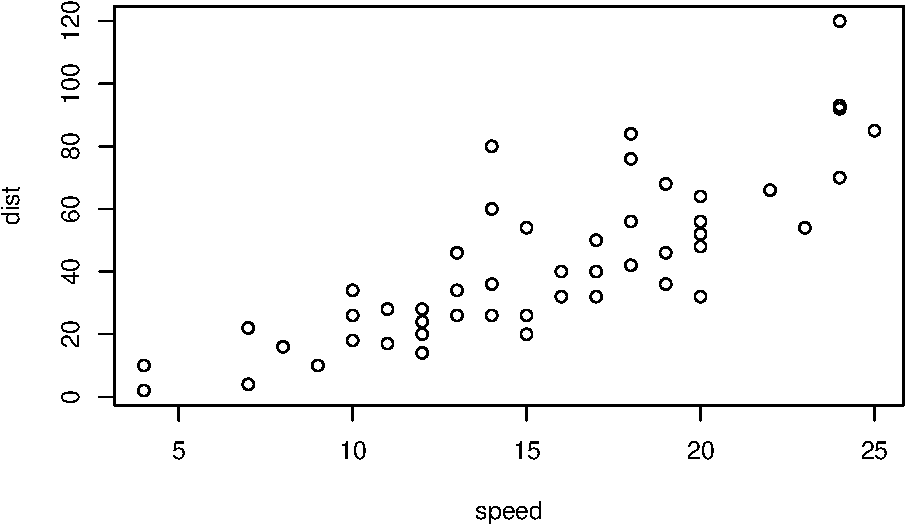
\includegraphics{./example_files/figure-latex/unnamed-chunk-3.pdf}
\caption{Exmple figure created by in-document R code.}
\end{figure}

As required by the APA guidelines, figures, too, are printed to the
final pages of the document.

\subsection{Citations}\label{citations}

You can insert citations like this:

\texttt{{[}e.g., @bauer\_2014; @bem\_2011{]}} → (e.g., {Baumer},
{Cetinkaya-Rundel}, {Bray}, {Loi}, \& {Horton}, 2014; Bem, 2011).

Citing without parentheses is, of course, also possible:

\texttt{@bauer\_2014} → {Baumer} et al. (2014).

The citation style is set in the header of this document with the
\texttt{csl} parameter. The relevant references will, of course, be
added to the documents references automatically. In order for citations
to work, you need to supply a .bib-file to the \texttt{bibliography}
parameter in the document header. See the
\href{http://rmarkdown.rstudio.com/authoring_bibliographies_and_citations.html}{RMarkdown
documentation} and \href{http://citationstyles.org/}{Citation Style
Language} for further details.

\subsection{Document options}\label{document-options}

This text is set as manuscript. If you want a thesis-like document you
can change the \texttt{classoption} in the document header from
\texttt{man} to \texttt{doc}. You can also preview a polished journal
typesetting by changing the \texttt{classoption} to \texttt{jou}.

Line numbering can be deactivated in by removing the \texttt{lineno}
argument from the header of this document.

\subsection{Last words}\label{last-words}

That's all I have. Enjoy writing your manuscript. If you have any
trouble or ideas for improvements, open an
\href{https://github.com/crsh/r2apa/issues}{issue} on GitHub or make a
pull request with the fix. ;)

\section{References}\label{references}

{Baumer}, B., {Cetinkaya-Rundel}, M., {Bray}, A., {Loi}, L., \&
{Horton}, N. J. (2014). R Markdown: Integrating A Reproducible Analysis
Tool into Introductory Statistics. \emph{ArXiv E-Prints}. Retrieved from
\url{http://adsabs.harvard.edu/abs/2014arXiv1402.1894B}

Bem, D. J. (2011). Feeling the future: experimental evidence for
anomalous retroactive influences on cognition and affect. \emph{Journal
of Personality and Social Psychology}, \emph{100}(3), 407---425.
doi:\href{http://dx.doi.org/10.1037/a0021524}{10.1037/a0021524}



\end{document}